\documentclass[a4paper,12pt]{scrartcl} 

%% \usepackage[latin1]{inputenc}
%%apt-get install texlive-lang-german kile kile-l10n  aspell-de  texlive-fonts-extra
%%damit ngerman keine Probleme mehr macht !!
\usepackage[utf8]{inputenc} 
\usepackage[T1]{fontenc}
\usepackage[ngerman]{babel}

\usepackage{setspace}

\setcounter{tocdepth}{3}				%Schatelungstiefe Inhaltsverz.
\usepackage[utf8]{inputenc}			%deutsche Umlaute
\usepackage{german, ngerman}
\usepackage[ngerman]{babel}			%Rechtschreibprüfung
\usepackage{color,listings} 			%Quellcode Highlighting, bindet das
\usepackage{float}					%% GRAFIKPOSITION MITTELS [H] ERWZINGEN
%Paket Listings ein
\usepackage{listings}
\usepackage{color}
\usepackage{textcomp}
\usepackage[T1]{fontenc}				%srccode
\usepackage[scaled]{beramono}		%srccode
\usepackage{longtable}				%mehrseitige tabellen
\usepackage[tableposition=b]{caption}
\usepackage[pdftex, pdftoolbar=false, hyperfootnotes=false, bookmarks,
bookmarksopen, bookmarksnumbered, bookmarksopenlevel=2, pdfpagelabels=true,
pdfstartpage=3, pdfstartview=FitH,]{hyperref} %Verlinkungen
\usepackage{array}					%farbige Tabellen
\usepackage[table]{xcolor} 			%farbige Tabellen
\usepackage{graphicx}				% \includegraphics bnoetigt dies

\usepackage{fancyhdr, graphicx}		%% Logo auf Titelseite
\renewcommand{\headrulewidth}{0pt}
\fancyhead[L]{}
\fancyhead[R]{
  \includegraphics[width=52mm]{./images/htwk.png}
}

%%%% mathemathische Formeln zentrieren und vom Text absetzen mittels \[ E = mc^2 \] anstatt $ E = mc^2 $ %%%%
\usepackage{amsmath}
\usepackage{amsthm}
\usepackage{amsbsy}
\usepackage{amssymb}


%java highliteting
\lstset {
  language=java,
  basicstyle={\footnotesize\ttfamily},
  numbers=left,
  numbersep=-5pt,
  numberstyle=\tiny\color{Gray},
  aboveskip=11pt,
  belowskip=11pt,
  showstringspaces=false,
  columns=flexible,
  keywordstyle=\color{Fuchsia},
  %identifierstyle=\color{Black},
  commentstyle=\color{ForestGreen},
  stringstyle=\color{blue},
  frame=single,
  breaklines=true,
  breakatwhitespace=true,
  tabsize=2,
  morekeywords={ }% <-- adding custom keywords
}
%%%%%%%%%%%%%%%%%%%%%%%%%%%%%%%%%%%%%%%%%%%%%%%%%%%%%%%%%%%%%%%

\definecolor{Navy}{rgb}{0,0,0.5}
\definecolor{Gray}{gray}{0.5}
\definecolor{dunkelgrau}{rgb}{0.8,0.8,0.8}
\definecolor{hellgrau}{rgb}{0.95,0.95,0.95}
\definecolor{hellgrau2}{rgb}{0.93,0.93,0.93}

\hypersetup{
	colorlinks=true, 			% false: boxed links; true: colored links
	linkcolor=Navy,          		% color of internal links
	citecolor=Gray,        			% color of links to bibliography
	filecolor=magenta,      		% color of file links
	urlcolor=blue,           			% color of external links
	linkbordercolor={1 1 1}, 		% set to white
	citebordercolor={1 1 1} 		% set to white
}


%Einrückung eines neuen Absatzes
\setlength{\parindent}{0em}

%Definition der Ränder
\usepackage[paper=a4paper,left=30mm,right=30mm,top=30mm,bottom=30mm]{geometry}

%Abstand der Fussnoten
\deffootnote{1em}{1em}{\textsuperscript{\thefootnotemark\ }}

%Regeln, bis zu welcher Tiefe (section,subsection,subsubsection) Überschriften angezeigt werden sollen (Anzeige der Überschriften im Verzeichnis / Anzeige der Nummerierung)
%\setcounter{tocdepth}{3}
%\setcounter{secnumdepth}{3}

\fancypagestyle{htwkheader}
{
   \fancyhf{}	% clear all header and footer fields
  \fancyhead[RO]{
	\makebox[\textwidth]{	%% schiebe Logo nach aussen auf den Rand
		\rule{1				%% nach aussen schieben hoeherer Wert -> Logo weiter nach aussen
		  \textwidth}{0cm} %% nicht nach unten schieben = 0cm
			\includegraphics*[width=52mm]{./images/htwk.png}	%%Logo HTWK
	  }
  }
}



\begin{document}
 
%Beginn der Titelseite
\begin{titlepage}
\begin{small}
\vfill {HTWK Leipzig\\
Fachbereich IMN \\
Sommersemester 2014}
\end{small}
 
\begin{center}
\begin{Large}
\vfill {\textsf{\textbf{
Traincard\\
}}}
\end{Large}
Beleg im Smartcard Programmierung\\bei Prof. Dr. rer. nat. Uwe Petermann
\end{center}
 
\begin{small}

\vfill
Kurt Junghanns, B.Sc.\\
Marcel Kirbst, B.Sc. \\
Michael Reher, B.Sc.\\
\\
\today
\end{small}
 
\end{titlepage}
%Ende der Titelseite
 
%Inhaltsverzeichnis (aktualisiert sich erst nach dem zweiten Setzen)
\tableofcontents
%Abbildungsverzeichnis und Tabellenverzeichnis auf einer Seite
\clearpage
\listoffigures
\listoftables
\thispagestyle{empty}
 
\clearpage
\onehalfspacing
 
\pagestyle{plain}
 
\section{Einleitung}
\label{sec:0}
Diese Arbeit befasst sich mit der Vorstellung der Belegarbeit im Fach Smartcard Programmierung mit dem Thema ``Traincard''. 
Ziel des Belegs ist die prototypische Implementierung eines Trainingssystems auf Basis JCOP-fähiger Smartcards. 
\\
\\
Im ersten Kapitel \nameref{sec:1} wird der Anwendungsfall für die prototypische Implementierung beschrieben, sowohl unter \nameref{subsec:1.1}, wie auch unter \nameref{subsec:1.2}. Im Kapitel \nameref{sec:2} werden die grundlegenden Technologien und Standards vorgestellt.  Kapitel \nameref{sec:3} erläutert detailliert die Systemumgebung, beschreibt den On-Card und den Off-Card Teil der Implementierung sowie deren Kommunikation. Abschließend wird im Kaptiel \nameref{sec:4} eine Einschätzung des Belegs gegeben. 

\clearpage
\section{Anwendungsfall}
\label{sec:1}
In Fitnessstudios werden heute noch bei der Neuanmeldung Trainingspläne auf Papier ausgegeben. Der Trainierende führt den Trainingsplan über die Trainingsperiode ständig bei sich und verzeichnet den Trainingsfortschritt in diesem Dokument.
Im Verlauf der Trainingsperiode kann der Trainer beurteilen, wie effektiv das Training beim Trainierenden ist.\\
\\
Die Verwendung von Trainingspläne auf Papier hat jedoch einige Nachteile. Beispielsweise wird das Dokument vom Trainierenden manchmal vergessen, die betreffenden Trainingsfortschritte müssen also nachgetragen werden. 
Weiterhin sind Traingspläne in Papierform nur bedingt resistent gegen Abnutzung und verschleißen mit fortdauernder Verwendung.
Um den genannten Nachteilen zu begegnen soll im Rahmen dieser Belegarbeit der Einsatz von Trainingsplänen
auf Basis so genannter Smartcards abgebildet werden. Smartcards können sehr leicht in einer Brieftasche mitgeführt werden und sind weniger anfällig für Abnutzung.
Weiterhin bieten sie weitere Vorteile wie automatische elektronische und anonyme Datenerfassung zu den Sportlern, die Möglichkeit die Daten extern zu sichern und bei Bedarf auf eine beliebige Smartcard zu exportieren.

\subsection{Anwendungsfall aus Sicht des Trainierenden}
\label{subsec:1.1}

Aus Sicht des Trainierenden bietet die Verwendung der Smartcard einige der folgenden Vorteile:
\begin{itemize}
\item leichte Transportierbarkeit
\item robuster als Trainingspläne aus Papier
\end{itemize}


\subsection{Anwendungsfall aus Sicht des Trainers}
\label{subsec:1.2}
Trainer profitieren beim Einsatz von Smartcards unter anderem von folgenden Vorteilen:
\begin{itemize}
\item leichte und lesbare Auswertung der vorgegebenen Trainingspläne
\item zusätzliche Metainformationen wie beispielsweise zu welchem Zeitpunkt welcher Datensatz geschrieben wurde
\item statistische Auswertungen lassen sich sehr leicht erstellen 
\item manipulationssicher
\item es fallen zusätzlich Metadaten an die ausgewertet werden können (z.B.: wann wurde die Karte an welchem Gerät benutzt)
\end{itemize} 


\clearpage
\section{Grundlagen}
\label{sec:2}
In diesem Kapitel wird auf die Grundlagen der in diesem Beleg verwendeten Technologien eingegangen.

\subsection{Grundlagen Smartcard}
\label{subsec:2.1}
Die in diesem Beleg verwendete Smartcard basiert auf der Java Card Technologie. Die Java Card Technologie bietet eine 
Teilmenge der Java Programmiersprache, sowie eine hinsichtlich der Anforderungen an Smartcards optimierte Laufzeitumgebung.

Die Verwendung von Java-basierten Smartcards bietet einige Vorteile, von denen nachfolgend eine Auswahl beispielhaft genannt sei: \cite{jcopdoc}

\begin{description}
\item[plattformunabhängig:] Java Card Applets, die der Java Card API entsprechen, lassen sich plattformunabhängig und herstellerübergreifend nutzen.
\item[Multiapplikationsfähig:] es können mehrere Applikationen gleichzeitig auf einer Smartcard ausgeführt werden
\item[hohe Flexibilität:] die Verwendung der objektorientierten Programmiersprache Java erlaubt die Erstellung komplexer Anwendungen für die Smartcard.  
\item[Post-Aktualisierbarkeit:] die Möglichkeit, nachträglich Code auf der Smartcard zu modifizieren und auszutauschen erhöht die Flexibilität weiter
\item[Standardkonformität:] die Java Smartcards entsprechen dem ISO7816 Standard \cite{iso7816}
\end{description}

Eine Java Smartcard besteht im Wesentlichen aus den Bestandteilen Kommunikationsschnittstelle, Speicher und einem Prozessor zur Durchführung von Berechnungen.
Bei Verwendung der Smartcard wird diese in ein Lesegerät eingelegt. Das Lesegerät wird in einschlägiger Literatur auch als Card Acceptance Device, abgekürzt CAD, bezeichnet.
Der Speicher auf Java Smartcards besteht aus zwei Typen, RAM und EEPROM. Der RAM-Speicher ist flüchtig und kann beliebig oft beschrieben werden. Der EEPROM-Speicher ist nichtflüchtig und kann nur endlich oft beschrieben werden, je nach Hersteller und Modell bis zu 100.000 mal pro Speicherzelle.  

\subsection{JCOP}
\label{subsec:2.2}
JCOP ist eine kontextorientierte Programmiererweiterung für die Programmiersprache Java und kombiniert COP-Vorteile mit neuen Konstrukten wie ereignisorientierten und deklarativen Layerkompositionen.

\subsection{APDU}
\label{subsec:2.3}

Die Kommunikation zwischen dem Kartenlesegerät und der Smartcard erfolgt reaktiv und paketweise. Reaktiv bedeutet, dass die Smartcard keine Kommunikation initiiert sondern nur auf Anfragen vom Lesegerät reagiert. Der bei der Kommunikation zwischen Smartcard und Lesegerät verwendete Kommunikationsmechanismus wird als Application Protocol Data Units, abgekürzt APDU, bezeichnet. Spezifiziert ist dies ebenfalls in ISO7816 Teil 4.\cite{iso7816}
\\

\begin{figure}[htb]
\begin{center}
 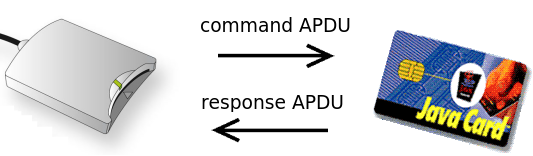
\includegraphics[width=1\hsize]{./images/apdu.png}
\end{center}
\caption[APDU-Kommunikation schematisch dargestellt, Quelle: Autoren]{\label{apdu}APDU-Kommunikation schematisch dargestellt, Quelle: Autoren}
\end{figure}

Die Kommunikation wird über ein so genanntes command APDU Paket initiiert, welches aus den folgenden Feldern besteht:


\begin{description}
\item[CLA:] class,gibt die Klasse an, spezifiziert ob es sich um ein ISO7816-4 konformes Kommando handelt
\item[INS:] gibt die Instruktion an
\item[P1:] zusätzlicher Parameter
\item[P2:] zusätzlicher Parameter
\end{description} 

Weiterhin können je nach Kommandotyp noch die folgenden, optionalen Felder an das command APDU Paket angehängt werden:


\begin{description}
\item[Lc:] Length, gibt die Länge der Kommandodaten
\item[Data:] gibt die Kommandodaten an
\item[Le:] gibt die Länge der erwarteten Antwort an
\end{description}

Als Antwort erhält das Lesegerät von der Smartcard ein so genanntes response APDU Paket. Dieses Antwortpaket kann Daten enthalten, dies ist jedoch nicht obligatorisch. 


\clearpage
\section{Umsetzung}
\label{sec:3}

Dieses Kapitel legt die Umsetzung dar.

\subsection{Kommunikation}
\label{subsec:3.0}

Die Anwendung besteht aus einem On-Card und einem Off-Card Teil.\\
Entsprechend der JCOP Umgebung, ist der On-Card Teil durch ein Applet realisiert, welches auf der Smartcard installiert und gestartet wird.
Diese Smartcard kann eine physische oder eine emulierte zum Einsatz kommen.
Im Rahmen dieses Projektes wird die Smartcard per JCOP Eclipse Umgebung emuliert und verwendet.
Dabei ist in der gestarteten JCOP Shell der Befehl $/close$ auszuführen, wodurch die Smartcard für externe  Zugriffe auf der lokalen IP des Emulator-Rechners auf dem Port 8090 erreichbar ist.

Der Off-Card Teil ist ebenfalls in Java geschrieben und kommuniziert mit Hilfe des OpenCard Frameworks mit der Smartcard.
\\

Die Kommunikation zwischen On-Card und Off-Card auf verschiedenen Rechnern benötigt entsprechende Regeln der Firewalls der Rechner, lokale Ausführung beider Teile auf einem Rechner hingegen keine.

Der Inhalt der APDUs orientiert sich stark an der Norm ISO 7816-4. Der konkrete Aufbau ist in Abbildung \ref{myapdu} dargestellt.\\
Die Abkürzungen stehen dabei für folgendes:
\begin{description}
\item[CLA] ein Byte, welches immer mit dem Wert 0 belegt wird, da die APDU nicht vollständig ISO 7816-4 konform ist
\item[INS] ein Byte, welches die Instruktion angibt
\item[NOA] ein Byte, welches die Anzahl an gesamt zu übertragenden APDUs zur vollen Abarbeitung der Instruktion angibt
\item[LEN] ein Byte, welches die Anzahl der folgenden Daten-Bytes aufzeigt
\item[DATA] beliebige Anzahl von Bytes, welche die Daten enthalten\footnote{Anzahl der Daten-Bytes sollte LEN entsprechen}
\item[SW1] ein Byte, welches den vorderen Teil der Statusrückgabe darstellt
\item[SW2] ein Byte, welches den zweiten Teil der Statusrückgabe enthält
\end{description}

Die Statusrückgabe wird automatisch durch die JCOP Umgebung an die APDU angehangen. Die Interpretation der Statusrückgabe ist anhand ISO 7816-4 durchzuführen.

\begin{figure}[htb]
\begin{center}
 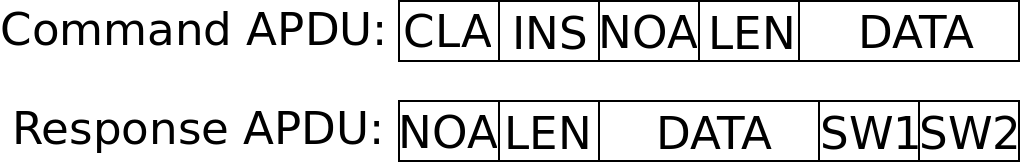
\includegraphics[width=1\hsize]{./images/myapdu.png}
\end{center}
\caption[Selbstdefinierter Dateninhalt der APDUs]{\label{myapdu}Selbstdefinierter Dateninhalt der APDUs}
\end{figure}

APDUs enthalten bis zu 256 Bytes, davon bis zu 252 Bytes für Daten.
Es sind ganze Trainingspläne und andere Objekte im Byte Format zwischen On-Card und Off-Card Teil zu übertragen. Dazu existiert pro Datenmodell in der dazugehörigen Klasse je eine Funktion zur Umwandlung von Instanz zu Byte Array und zur Erzeugung einer Instanz aus einem Byte Array. Diese Umwandlung  wurde eigens implementiert und orientiert sich am Aufbau von Ethernet Paketen. Ein Paket oder Byte Array besteht dabei immer aus einem Byte für einen eindeutigen Identifikator des Modells, zwei Bytes für die Anzahl der folgenden Bytes sowie Daten Bytes.
Eine Instanz des Modells MyDate mit den Attributen Jahr\footnote{Bei einem Jahr werden nur die letzten zwei Ziffern hexadezimal abgespeichert.}, Monat und Tag wird in folgendes Byte Repräsentation umgewandelt: $01$ $00$ $03$ $0e$ $07$ $0b$
\\

%verschlüsselung
Bei der Realisierung des Trainingssystemes werden keine Sicherheitsrelevanten Daten zwischen On-Card und Off-Card Teil übertragen. Auf Grund dessen wurde auf eine verschlüsselte Kommunikation mit asymmetrischer oder symmetrischer Verschlüsselung verzichtet.
Einzig Rollen-spezifische Schreibvorgänge sind in beiden Card Teilen durch je ein Passwort geschützt.
Der Trainer und der Sportler besitzen jeweils ein Passwort, welches mit der Java Bibliothek java.security.MessageDigest und derdarin enthaltenen  Hashfunktion SHA-256 zu einem 32 Byte langem Wert gehasht.
Dieser Hash ist auf der Smartcard gespeichert und muss bei der Anmeldung zum anschließenden Vergleich des Trainers oder Sportlers übertragen werden.
Der jeweilige Benutzer gibt in der grafischen Oberfläche sein Passwort im Klartext ein worauf die Programmlogik dieses hasht und es an die Smartcard überträgt.
Initial ist die Karte mit je einem Hash für Trainer und Sportler zu füllen. Im Zuge der Vereinfachung sind diese Werte bereits statisch gefüllt.
Um den Passworthash des Trainers zu setzen ist das in Listing \ref{•} dargestellte Kommando an die Smartcard zu senden.

\begin{lstlisting}
			\send 00 02 00 00 04 00 00 42 83 //Add Element with ID 00 00 42 83
			Response:
			Success: 90 00
			Failure: 6A 83
		\end{lstlisting}

\subsection{Datenstruktur}
\label{subsec:3.1}
Die Übersicht der Modellklassen ist in \nameref{off-card} zu sehen.
\\

Die Datenmodelle bilden die auf der Smartcard gespeicherten bzw. die vom Off-Card Teil verwendeten Datensätze wieder.
Jede Modellklasse besitzt einen statischen Identifikator, einen Konstruktor, welcher alle Klassenvariablen setzt, und öffentliche lese- und Schreibmethoden der einzelnen Klassenvariablen.
Weiterhin leitet jede Modellklasse von der abstrakten Klasse IModel ab, wodurch die Methoden toBytes und fromBytes überschrieben werden müssen und diese somit bei allen Klassen verfügbar sind.
\\

Jeder Trainingsplan, hier Workoutplan, besitzt die folgenden Attribute:
\begin{itemize}
\item Erwärmungsphase
\item Trainingsphase
\item Abkühlungsphase
\item Startdatum
\item Enddatum
\end{itemize}
Jede Phase ist dabei ein Menge von Übungen bzw. Stages.
\\

Eine Übung ist aus folgenden Attributen aufgebaut:
\begin{itemize}
\item Tagesnummer
\item Geräteidentifikator
\item Muskelgruppenidentifikator
\item Übungsnummer
\item Menge von Sätzen, hier Sets
\end{itemize}
Die Tagesnummer gibt an, welcher Trainingstag des wochenbezogenen Trainingsplanes die Übung zugeordnet ist.
Da Zeichenketten nicht direkt auf der Smartcard gespeichert werden können, bzw. deren Byterepräsentation bei Beschreibungen die APDU Grenze von 256 Byte ohne Weiteres überschreiten können, werden zu Geräten und Muskelgruppen nicht deren Namen und Beschreibungen, sondern nur ein Identifikator gespeichert. Dieser Identifikator kann im Off-Card Teil zu einer Zeichenkette umgewandelt werden.
\\

Einzelne Sätze beinhalten die Satznummer, das zu verwendende Gewicht und die Anzahl der Wiederholungen mit dem Gewicht.
\\

Ein Datum wird durch die Klasse MyDate repräsentiert, welche je ein Byte für Jahr, Monat und Tag enthält.
\\

Die Fortschrittsdarstellung erhebt deren Daten aus einer Menge von Fortschrittselementen mit den folgenden Attributen:
\begin{itemize}
\item Übungsnummer
\item letzter Übungswert
\item bester Übungswert
\item schlechtester Übungswert
\end{itemize}
Ein Übungswert enthält dabei das verwendete Gewicht, die durchgeführten Wiederholungen und den Tag an welchem die Übung mit dem Gewicht und den Wiederholungen durchgeführt wurde.

\subsection{On-Card Teil}
\label{subsec:3.2}
Der On-Card Teil wird durch das Applet $Traincard$ repräsentiert.
\\


Im Klassendiagramm in der Abbildung \ref{diaoncard} ist das Applet mit dessen Klassenvariablen und Methoden dargestellt.
Das Applet befindet sich im Package\\htwk.smartcard.traincard und muss auf der verwendeten Smartcard installiert und gestartet werden.
\\

Entsprechend der Oberklasse javacard.framework.Applet, existieren Methoden, welche die Installation, Ausführung und Deselektion behandeln.
Die wichtigste Methode ist dabei process, welche ankommende APDUs erhält, diese auswertet, die entsprechende Klassenmethode aufruft und deren Antwort-Bytes in Form einer Response APDU zurücksendet.

\begin{figure}[htb]
\begin{center}
 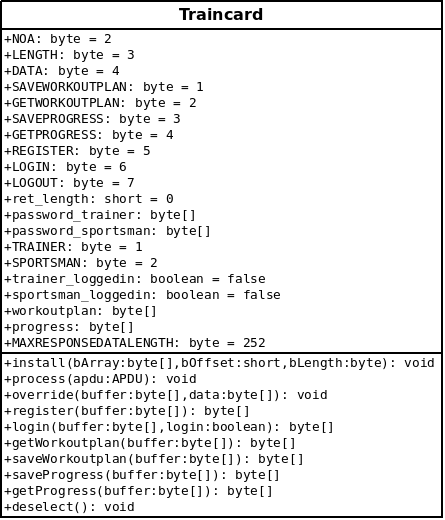
\includegraphics[width=.7\hsize]{./images/Klassendiagramm_oncard.png}
\end{center}
\caption[Klassendiagramm On-Card Teil]{\label{diaoncard}Klassendiagramm On-Card Teil}
\end{figure}


%das applet empfängt anfragen, wertet diese aus und sendet Daten oder ein erfolgsbyte im datenbereich zurück
%Daten werden dabei immer als byte arrays geschrieben und gelesen

%passwörter sind gehashed abgelegt

Das Instruktionsbyte wird mit den statischen Konstanten verglichen und anhand eines Treffers die entsprechende Methode aufgerufen. Jede dieser Methoden erhält den Puffer der APDU und gibt ein Byte Array für den Puffer der Response APDU zurück.
Der Aufbau der Command und Response APDU ist in der Abbildung \ref{myapdu} dargestellt.
Die darin dargestellten Data Bytes sind entsprechend der jeweiligen Instruktion gefüllt.\\
$00$ $02$ $01$ $01$ $01$ als APDU liest beispielsweise den Trainingsplan und sendet ihn zurück. Ist der Trainingsplan größer als MAXRESPONSEDATALENGTH Byte, muss mit $00$ $02$ $01$ $01$ $02$ eine weitere APDU mit den nächsten Bytes des Trainingsplanes angefordert werden.
\\

Lokale Byte Arrays der Methoden werden stets flüchtig mit der Methode makeTransientByteArray der Klasse javacard.framework.JCSystem angelegt.
Der Vergleich und das Kopieren von Byte Arrays erfolgt mit den Methoden arrayCompare und arrayCopy der Klasse javacard.framework.Util.
Dadurch wird der EEPROM der Smartcard nicht durch Schreibvorgänge belastet und die Ausführungszeit verringert sich.
\\

Der Trainingsplan und der Fortschritt wird in dynamischer Größe auf der Smartcard gespeichert und bei jedem Schreibvorgang neu erzeugt.


\subsection{Off-Card Teil}
\label{subsec:3.3}

% der offcard Teil besteht aus der graphischen Oberfläche, der Logik zur Steuerung der Oberfäche und der Logik zur Kommunikation mit der Smartcard
%screenshots mit erklärungen was gemacht wird + grob technisches
%passwörter werden gehashed
%Packagediagramm

Der Inhalt dieses Abschnittes bildet die Umsetzung des Off-Card-Teils. Dabei wird auf die graphische Oberfläche, die Logik zur Steuerung und zur Kommunikation mit der Smartcard eingegangen. \\
\newline
Wenn man die Off-Card-Anwendung startet, gelangt man in das Hauptmenü der Anwendung, welches in der Abbildung \ref{main}  dargestellt ist. Dieses Menü enthält fünf Buttons, welche jeweils zu einer Funktion des Programmes führt. Den gesamten Trainingsplan, den Tagesplan und den Trainingsfortschritt kann man sich ohne Eingabe eines Passwortes anschauen. Um die Trainingsergebnisse einzutragen oder den Trainingsplan zu ändern, ist ein Passwort nötig. Jede der Funktionen, sowie die Passwortabfrage, wird im folgenden genauer erläutert.

\begin{figure}[h]
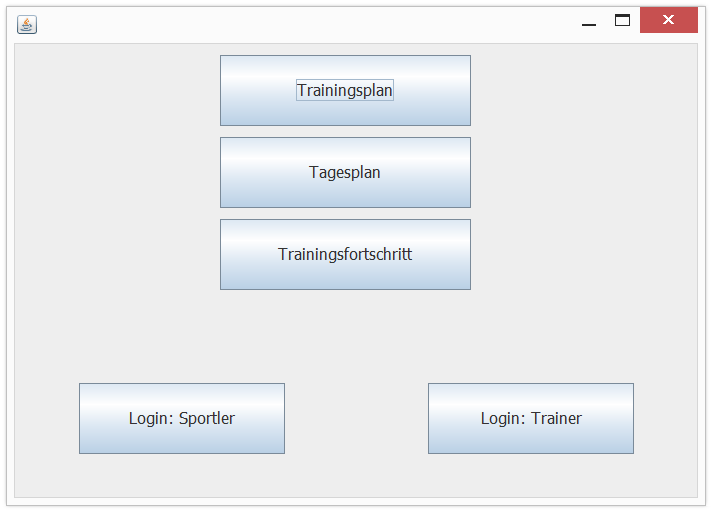
\includegraphics[width=1\hsize]{./images/main.png}
\caption{Hauptmenü}
\label{main}
\end{figure}

\newpage

\subsubsection*{Trainingsplan}

Über den Button Trainingsplan gelangt man in die nächste Ansicht, welche den gesamten aktuellen Trainingsplan darstellt (Abb. \ref{main}). Um den Trainingsplan zu laden, ruft das Programm die Funktion CardInterface.getWorkoutplan() aus dem CardInterface auf, welche als Rückgabewert den aktuellen Trainingsplan liefert. Dieser wird im Anschluss ausgelesen und in die Tabelle geschrieben. Wenn der Trainingsplan leer ist, ist folglich auch die Tabelle leer. Über den Zurück Button gelangt man, wie auch in allen anderen Funktion, zurück in das Hauptmenü.

\begin{figure}[h]
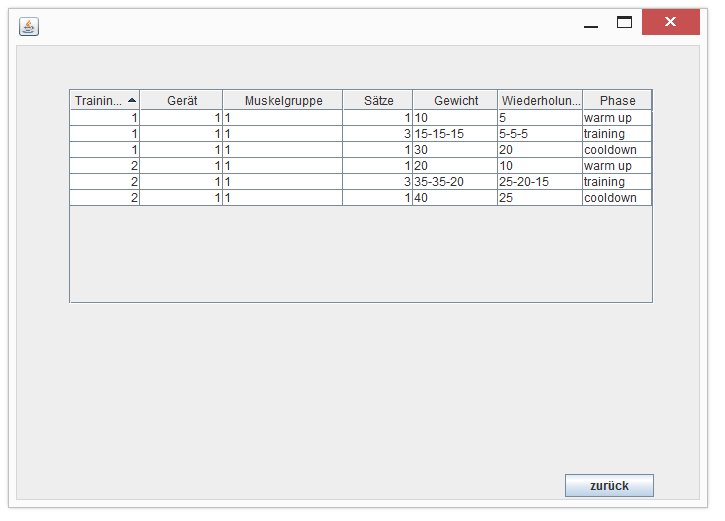
\includegraphics[width=1\hsize]{./images/gesamt.png}
\caption{gesamter Trainingsplan}
\label{main}
\end{figure}
\newpage
\subsubsection*{Tagesplan}

Die Ansicht des Tagesplan ist ähnlich zur Anzeige des gesamten Trainingsplans, mit einer Einschränkung. Über die Combobox "'Tag"' kann der gewünschte Tag ausgewählt werden. Nach dieser Auswahl wird in der Tabelle, welche den Trainingsplan anzeigt, nur diejenigen Übungen eingetragen und dargestellt, welche an dem jeweiligen Tag ,laut Trainingsplan, stattfinden sollen. Dazu besitzt jede Stage in einem Workoutplan-Object ein Attribut day. Diese Ansicht ist in Abbildung \ref{day} zu sehen.

\begin{figure}[h]
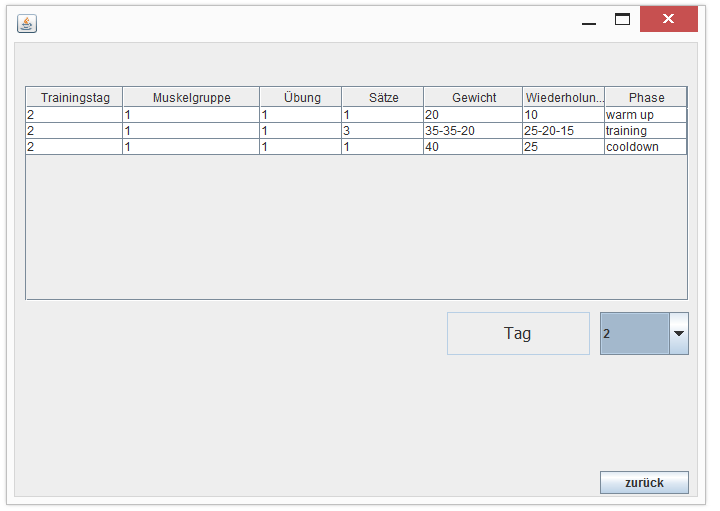
\includegraphics[width=1\hsize]{./images/tag.png}
\caption{Tagesplan}
\label{day}
\end{figure}
\newpage
\subsubsection*{Login: Trainer}

Um einen Trainingsplan mit den beiden Funktionen Trainingsplan und Tagesplan anzeigen zu können, ist es zuvor notwendig, einen Trainingsplan zu erzeugen. Dies ist möglich, wenn man sich als Trainer einloggt, wozu eine Passworteingabe nötig ist (Abb. \ref{login}).

\begin{figure}[h]
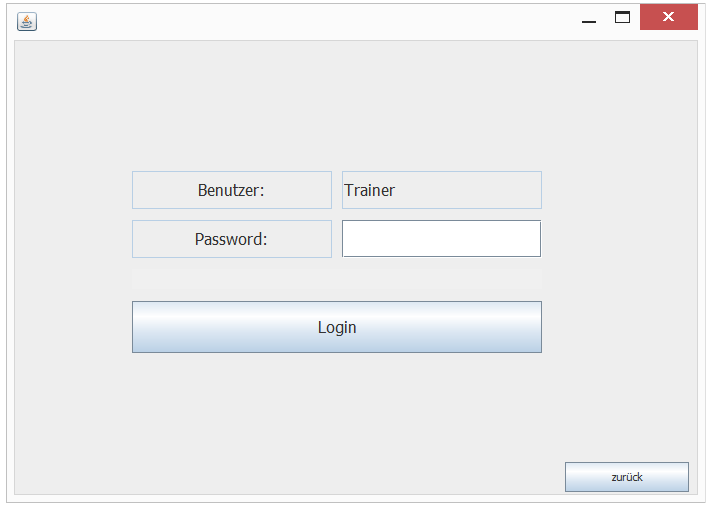
\includegraphics[width=1\hsize]{./images/login.png}
\caption{Eingabemenü des Trainers}
\label{login}
\end{figure}
\newpage
Wenn man sein Passwort eingegeben hat und auf Login drückt, wird das Passwort gehashed und an die Smartcard mit dem Benutzertyp (Trainer oder Sportler) gesendet. Diese überprüft das Passwort auf Korrektheit und gibt als Antwort true oder false zurück. Wenn das Passwort korrekt ist, gelangt man in die Traineransicht und kann den aktuellen Trainingsplan verändern oder einen neuen anlegen. Die Ansicht ist in Abbildung \ref{trainer} dargestellt. Über den Button neue Übung können weitere Zeilen zur Tabelle hinzugefügt werden. Zusätzlich zu den Übungen kann ein Start und Enddatum für diesen Trainingsplan festgelegt werden. Da auf der Karte keine Strings gespeichert werden können, muss man mit ID's arbeiten. Diese ID's kann man dann im Off-Card-Teil über eine Hashmap speziellen Strings zuweisen um beispielsweise die Muskelgruppe nicht, wie in der Abb. \ref{trainer} zu sehen ist, als Zahl darstellen zu müssen. Beim speichern des Trainingsplans wird die Tabelle ausgelesen und die entsprechenden Werte einem neuen Workoutplan-Objekt zugewiesen, welches auf der Smartcard gespeichert wird. Zusätzlich dazu wird, auch ein neues Progressarray auf der Karte erzeugt, welche alle Stage-ID's für den neuen Plan enthält. Dies ist notwendig um den Fortschritt des Sportlers eintragen, speichern und auslesen zu können.

\begin{figure}[h]
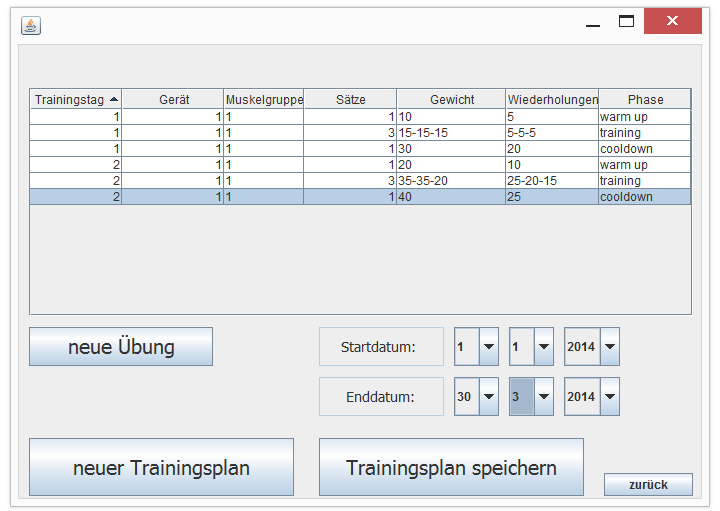
\includegraphics[width=1\hsize]{./images/Trainer.png}
\caption{Eingabemenü des Trainers}
\label{trainer}
\end{figure}


\newpage
\subsubsection*{Login: Sportler}

Wenn nun ein Trainingsplan erzeugt und abgespeichert wurde, kann der Sportler seine Trainingsdaten bezüglich dieses Plans eintragen. Dazu ist es notwendig, das er sich als Sportler einloggt. Wenn der Benutzer als Sportler angemeldet ist, gelangt er in die Sportleransicht, welche in Abb. \ref{sportler} zu sehen ist. In dieser Ansicht werden alle Übungen, für den ausgewählten Tag, angezeigt. Die Auswahl geschieht nach dem gleichen Prinzip, welches auch in der Tagesplanansicht benutzt wird, siehe Abschnitt Tagesplan. Die Daten zu den jewieligen Übungen, kann der Nutzer manuell eingeben, oder die vorgegebenen Trainingswerte über die Checkbox übernehmen lassen. Wenn die Daten eingetragen sind und gespeichert werden (Button: Trainingsdaten speichern), wird das Progressarray aktualisiert. Dazu wird es zunächst von der Karte gelesen, dann Werte die eingetragenen Werte überprüft, ob gegebenenfalls ein neuer bester oder schlechtester Wert erreicht wurde. Nach der Aktualisierung wird das Progressarray wieder auf der Karte abgelegt. 

\begin{figure}[h]
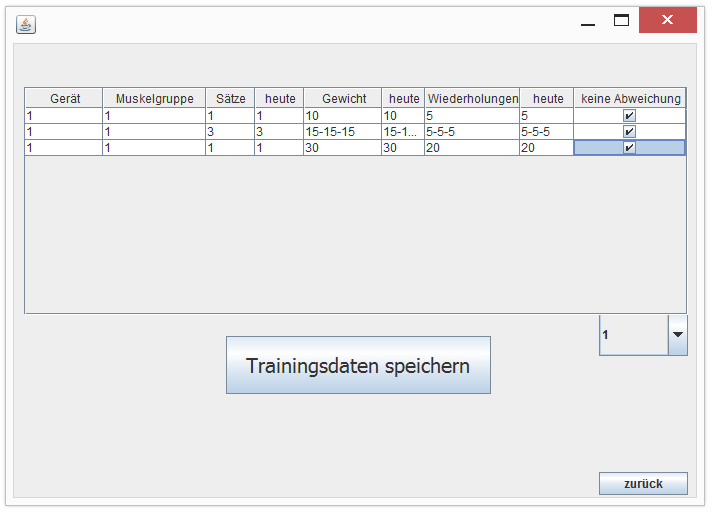
\includegraphics[width=1\hsize]{./images/sportler.png}
\caption{Eingabemenü des Sportlers}
\label{sportler}
\end{figure}
\newpage
\subsubsection*{Trainingsfortschritt}

In der Funktion Trainingsfortschritt wird der aktuelle Trainingsfortschritt angezeigt. Dazu wird von der Karte der aktuelle Trainingsplan und das Progressarray abgerufen. Dabei gibt es verschiedene Möglichkeiten. Zum einen kann noch kein Trainingsplan existieren. Wenn dieser Fall vorliegt, bleibt die Tabelle leer und das Progressarray existiert folglich nicht und muss nicht ausgelesen werden. Wenn ein Trainingsplan existiert, allerdings noch keine Trainingsdaten eingetragen wurden, wird nur der Trainingsplan abgebildet und die Felder der Trainingsdaten bleiben leer, siehe Abb. \ref{empty}.

\begin{figure}[h]
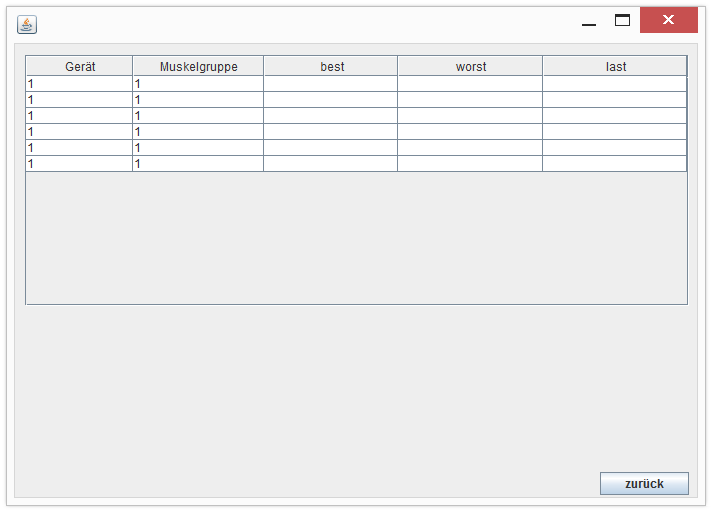
\includegraphics[width=1\hsize]{./images/fortschritt-leer.png}
\caption{Trainingsfortschritt ohne Einträge}
\label{empty}
\end{figure}
\newpage
Weiterhin exisitiert die Möglichkeit, das im Progressarray zu einigen Übungen schon Trainingsdaten vorhanden sind, allerdings noch nicht zu allen. Dann werden, wie in der Abbildung \ref{full} zu sehen ist, alle vorhandenen Werte eingetragen und die restlichen freigelassen. Die Spalte best bzw. worst gibt jeweils den besten bzw. schlechtesten Trainingswert an. Wenn ein neuer Trainingswert eingetragen wird, wird dieser immer in der Spalte last abgebildet. Um im späteren Verlauf nachvollziehen zu können, wann welcher Wert erreicht wurde, wird bezüglich der Daten noch ein Datum angegeben.

\begin{figure}[h]
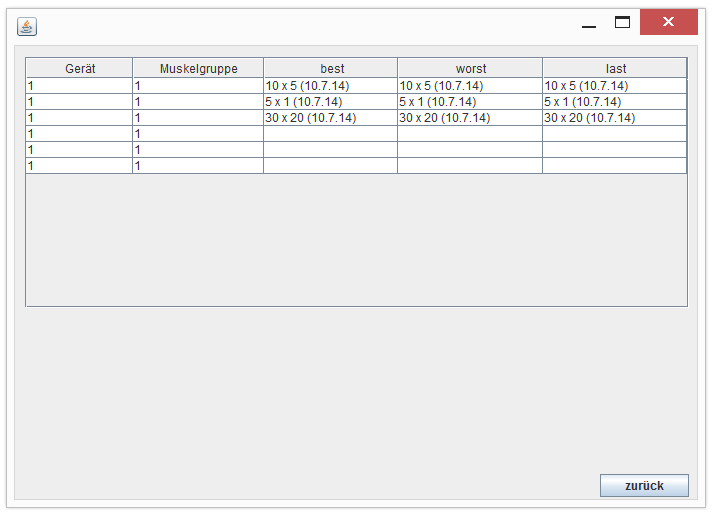
\includegraphics[width=1\hsize]{./images/fortschritt-mit-eingabe.png}
\caption{Trainingsfortschritt mit Einträgen}
\label{full}
\end{figure}
\newpage
\subsubsection*{Klassendiagramm Off-Card Teil}

In diesem Abschnitt wird das Klassendiagram der Traingui beschrieben.\\
\newline
Die Traingui ist in die vier packages: model, main, gui und comm unterteilt. Im package main befindet sich die main Methode in der Klasse Traingui, welche als erstes die MainView startet, um das Hauptmenü anzuzeigen. Von diesem aus, sind alle weiteren Funktionen erreichbar, welche in den vorangegangen Abschnitten erläutert wurden.\\
\newline
Die MainView befindet sich im package gui, welche alle Views (MainView, SportlerView, FortschrittView, TagesplanView, TrainerView und TrainingsplanView) und die Programmlogik (TableMethods und PasswordCheck) enthält. Die Logik dient zum Auslesen und Schreiben der Workoutplans und Progress Elementen, was in der Klasse TableMethods implementiert ist. Das Auslesen dient zum Befüllen der Tabellen. Vor dem schreiben neuer Elemente ist es notwendig, die Tabellen auszulesen und die entsprechenden Werte in das jeweilige Objekt zu übertragen. Die Zugriffsrechte auf die Smartcard werden auf Benutzerseite über die Klasse PasswortCheck geregelt, welche die eingegebenen Passwörter an die Smartcard überträgt und diese dann die Eingabe aus Korrektheit überprüft. \\
\newline
Jegliche Kommunikation der Traingui zur Smartcard, wird mit dem package comm realisiert. Dies beinhaltet dazu die Klassen CardInterface und CardHandler, welche alle benötigten Funktionsaufrufe, zum lesen und schreiben von und auf die Karte, enthalten.\\
\newline
Der Aufbau der Datentypen ist im package model deklariert. Dieses enthält ein Interface IModel und die jeweiligen Klassen für den einzelnen Elemente: Workoutplan, Progress, ProgressElement, MyDate, Stage, und Set. Die Klasse MyDate wird benötigt, da die Karte kein Date-Objekt speichern kann und für das Ablegen von einem Datum eine Byte-Kodierung benötigt.


\begin{figure}[h]
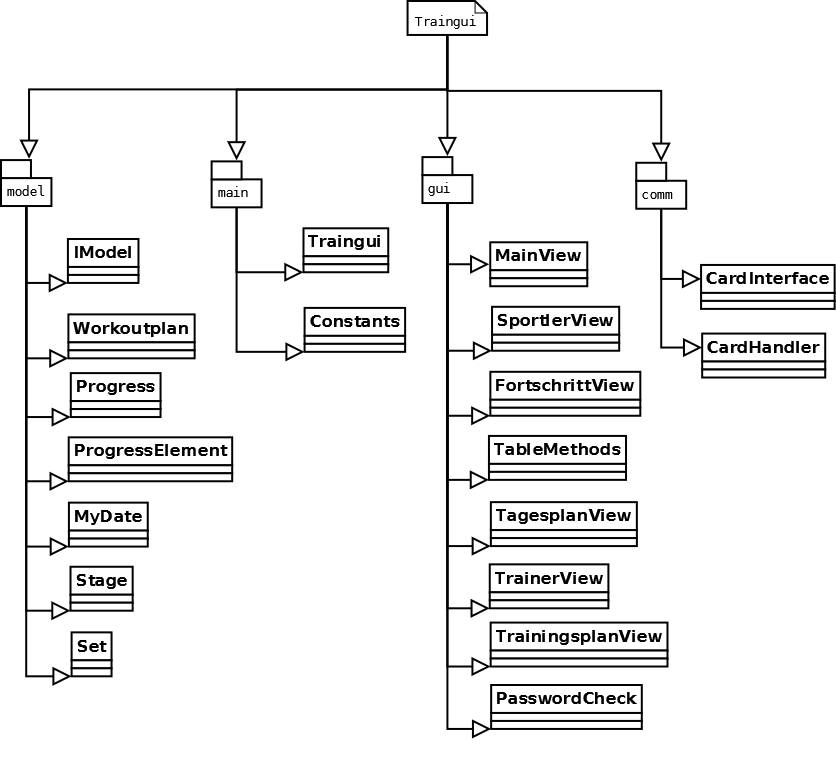
\includegraphics[width=1\hsize]{./images/Diagramm1.png}
\caption{Klassendiagramm Off-Card Teil}
\label{off-card}
\end{figure}



\clearpage
\section{Zusammenfassung und Ausblick}
\label{sec:4}
Der beschriebene Anwendungsfall wurde im Rahmen dieses Belegs analysiert und eine Lösung implementiert. 

- ziel kurz beschreiben -> wurde erreicht
- wie wurde das ziel erreicht
- AUSBLICK
- github

Im Rahmen dieses Beleges sollte ein On-Card und ein Off-Card Teil erstellt werden, welche ein Trainingssystem für einen Trainer und einen Sportler bereitstellen.
Dabei sollen die Elemente Trainingsplan, Trainingsfortschritt und Tagesplan im Rahmen der Benutzerrollen verfügbar und veränderbar sein.
\\
Dieses Ziel wurde erreicht. Der Programmcode wurde implementiert, die Programmteile sind funktionsfähig und eine entsprechende Dokumentation liegt vor.
\\
Die Anforderungen wurden zu Beginn definiert und stellten die Grundlage der folgende Modellierung dar.
Die Modelle und die Programmstruktur bildeten die Grundlage für die anschließende Programmierarbeit und die Erstellung der Dokumentation.
Weiterhin ermöglichte dieses Vorgehen eine gleichberechtigte Arbeitsteilung.
\\


\clearpage
\section{Quellenverzeichnis}
\label{sec:6}

%%empty command removes double title
\renewcommand\refname{}
%%%%


\begin{thebibliography}{999}
\bibitem{uwe}Prof. Dr. rer. nat. Petermann, Uwe: {\sl Lehrmaterial zur Veranstaltung Smartcard-Programmierung im SS2014 an der HTWK-Leipzig.}\\
\url{https://bildungsportal.sachsen.de/opal/auth/RepositoryEntry/437649412/CourseNode/87246817112798}\\
intern abrufbar am 10.Juli 2014

\bibitem{jcopdoc}Sun Microsystems, Inc.:  {\sl Java Card Applet Developer's Guide}\\
\url{http://www.oracle.com/technetwork/java/javacard/downloads/index.html}\\
abrufbar am 01.Juli 2014

\bibitem{iso7816}International Organization for Standardization:\\
{\sl ISO 7816 - Identification cards -- Integrated circuit cards}\\
kostenpflichtig abrufbar unter \url{http://www.iso.org/}

\end{thebibliography}
\end{document}